\chapter{Methods}

From a computer science (informatics) point of view, it is assumed that the processing of medical information is, in general, a computational problem, which is understood as a task that can be solved by a computer. An algorithm is a set of operations that is used to accomplish tasks and solve problems. 
The important features of an algorithm are effectivity (what is the time complexity of the algorithm regarding the size of input data) and scalability (how far can an algorithm benefit from parallel computing). Grid computing and cloud computing brings a technology that enables parallel computing in a large amount of shared computers, servers or cluster of servers introduces large speedup of computation and can decrease the time of computation substantially. However, problems solvable by algorithms with exponential time complexity (e.g. NP-hard or NP-complete\nomenclature{NP-complete}{Nondeterministig Polynomial - complete}) can't be addressed by any large scale infrastructure \cite{Garey1979}. Therefore, additional non-exact methods for such type of problems are used to obtain at least some solution including heuristic method (eliminate some steps or solution classes that seems to not go to optimal solution), randomization (pseudo random values are generated and statistical methods can be used to compute expected optimal value) and others. 

\section{Sharing Medical Images}
The DICOM standard\footnote{DICOM: \url{http://dicom.nema.org/} accessed January 2015}\nomenclature{DICOM}{Digital Imaging and Communication Protocol} was used as a joint protocol to integrate grid-based system Globus MEDICUS \cite{Erberich2006} with current production system MEDIMED for sharing medical images among different hospitals \cite{Slavicek2010}, which is based on common distributed system with central cluster. 
% which may suffer with single point of failure and bottleneck issues. 
Globus MEDICUS \cite{Erberich2006,Erberich2007} implements a DICOM Grid Interface Service (DGIS) and integrates the open-source PixelMed\texttrademark ~Java DICOM Toolkit\footnote{\url{http://www.pixelmed.com/} accessed February 2015} into a web service, communicating via the DICOM protocol. Furthermore, it forwards queries to the underlying services within Globus toolkit. The console application of the MEDIMED project can be interconnected via DICOM protocol with local Picture Archiving and Communication System (PACS)\nomenclature{PACS}{Picture Archiving and Communication System} and selected DICOM studies can be sent/retrieved to another institution connected to the MEDIMED project.




%The typical workflow of a medical image in a hospital is in Figure \ref{fig:pacs}. 
%\begin{figure}[ht]
%    \centering
%    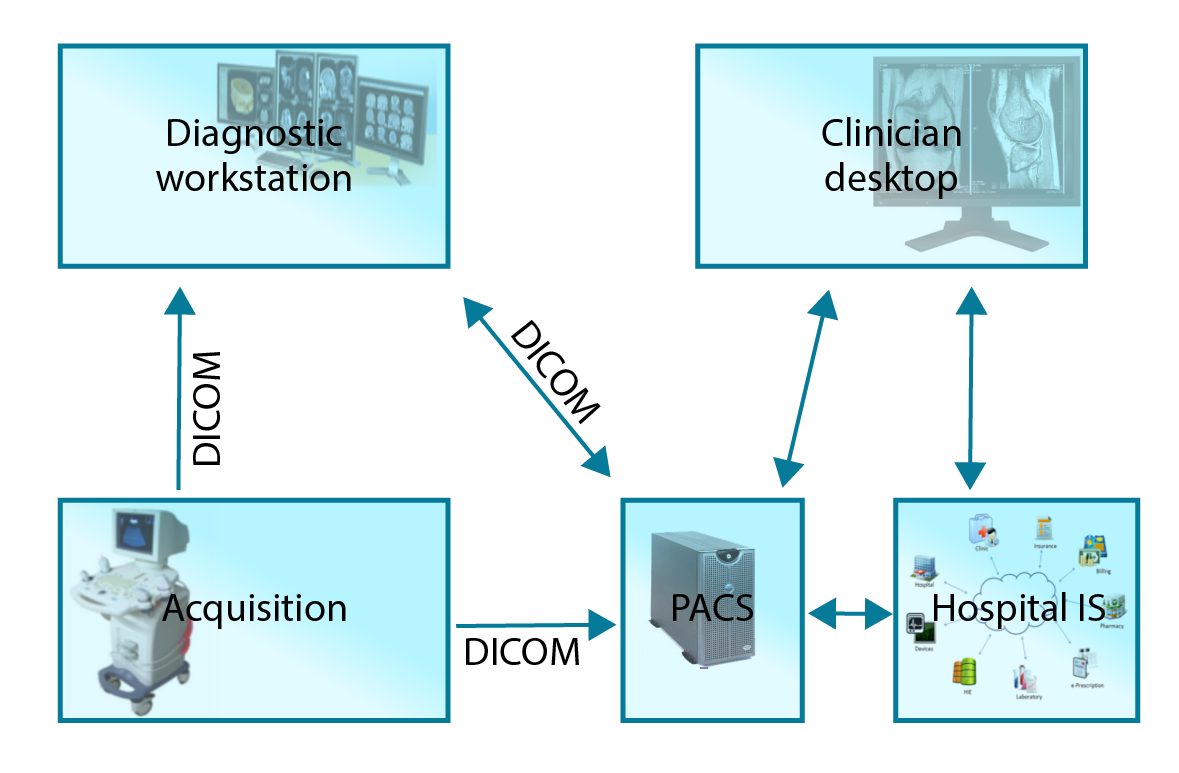
\includegraphics[width=0.7\textwidth, height=8cm]{img/chapter3-pacs.png}
%    \caption{Data acquisition is made by modalities (magnetic resonance, ultrasonography, etc.). By using the DICOM format and protocol, it can be directly transferred and visualized by diagnostic workstation. With the metadata filled by an expert physician, the image is stored in PACS. Other desktops within the hospital can retrieve the image and review the report.}
%    \label{fig:pacs}
%\end{figure}
%When there is need to share medical data records including medical images among different institutions and hospitals, a challenge should be solved with data confidentiality and size of the data. The DICOM\footnote{DICOM: \url{http://dicom.nema.org/} accessed January 2015}\nomenclature{DICOM}{Digital Imaging and Communication Protocol} standard is used for exchanging medical images electronically.  Picture Archiving and Communication System (PACS)\nomenclature{PACS}{Picture Archiving and Communication System} holds the acquired DICOM images with metadata and description, which are  noted by experts. PACS is usually part of the information systems in hospitals.
%
%

%\section{Sharing Medical Images}
%Various tools are already available within current grid infrastructures, including open-source and licensed software for computation. The local scientific grid provider may give a list of the available applications\footnote{applications available in CESNET METACENTRUM \url{https://wiki.metacentrum.cz/wiki/Kategorie:Applications} accessed February 2015}. Alternatively, application databases are available in a broader environment, e.g., in the EGI.eu application database\footnote{\url{https://appdb.egi.eu/} accessed February 2015}.
%Additionally, the workflow systems and scientific gateways that are mentioned in section \ref{sec:introworkflow} try to hide the complexity of grid or cloud computing infrastructures and may also be used to integrate specific domains.
%In designing a new application, the programming model of parallel computing and/or distributed  computing (in section \ref{sec:parallelprogramming} and  \ref{sec:distributedprogramming}) needs to be followed, utilizing the benefits of grid computing and cloud computing.

%The general approach to port applications to a grid infrastructure is to automatize what can be automatized, i.e., make scripts, configure system, prepare some user interface, integrate with existing applications, utilize protocol compatibility, etc. Additionally, the prepared template, script or application should be reused for further similar computational requests.

%\section{Sharing Medical Images}
%\label{sec:imaging}
%
%Use cases that relate to digital medical images involve image acquisition, preprocessing, storing and searching \cite{Bankman2000}.
%
%The acquisition of a medical image is performed with different modalities (different types of equipment and sensors) by radiologists or other specialists. The DICOM\footnote{DICOM: \url{http://dicom.nema.org/} accessed January 2015}\nomenclature{DICOM}{Digital Imaging and Communication Protocol} format and protocol has become an industrial standard for exchanging medical images electronically and in Picture Archiving Communication Systems (PACS). PACS holds the acquired DICOM images with metadata and description, which are  noted by experts. PACS is usually part of the information systems in hospitals. Figure \ref{fig:pacs} shows the typical workflows of a medical image in a hospital.
%
%
%
%%To summarize this section, in past years, 
%Digital medical image acquisition, storing, exchanging and processing has become common and it currently uses distributed computing techniques\cite{Slavicek2010, Ross2010, Saliba2012}. Several efforts have been made to implement medical data management within grid or cloud infrastructures for research purposes\cite{Erberich2006, Duque, Montagnat2007, Krefting2009, Krefting2010}  and to integrate them with production infrastructures \cite{Skaburskas2008, Benkner2010} or to share knowledge in semi-formally described semantics \cite{Kuba2006}.
%
%The Globus toolkit belongs to a group of the most used grid middleware (see section~\ref{sec:servicegrid}). 
%%The core service included in Globus Toolkit is GridFTP -- grid extension to file transfer protocol(FTP)\nomenclature{FTP}{File Transfer Protocol}. This implements strategies such as \emph{stripping data} into multiple pieces; the \emph{parallel transfer of data}, utilizing stripped data parts to be transferred via different channels; \emph{partial file transfer}, some applications may not need to access the whole file but rather a smaller portion of it, etc., as described by Foster et al. and Allcock et al. \cite{Foster2006, Allcock2005}. Other core services are Replica Location Service, which aims to localize data, and Globus Resource Allocation Management (GRAM), which provides web service and proxies to the lower level job scheduler's implementation \cite{Foster2006}.
%%Next to core services, the domain-specific services might be implemented for the purpose of an application that uses the Open Grid Service Architecture (OGSA). 
%Globus MEDICUS \cite{Erberich2006,Erberich2007} implements a DICOM Grid Interface Service (DGIS) and integrates the open-source PixelMed\texttrademark ~Java DICOM Toolkit\footnote{\url{http://www.pixelmed.com/} accessed February 2015} into a web service, communicating via the DICOM protocol. Furthermore, it forwards queries to the underlying services within Globus toolkit. 
%
%%DGIS acts as a gateway to a grid infrastructure. As communication via the DICOM protocol is not secured, it is recommended that the DGIS be installed on the location of the PACS system or the DICOM ready modality or software. When a DICOM study is uploaded into DGIS, it is anonymized and stored. A record is made into another service’s Meta Catalog service, which resides in the same domain or anywhere in the grid that is accessible via the Globus Toolkit. Such an anonymized database of DICOM records can be used to query via the DGIS interface and to, for example, integrate with web-based applications, showing records for research purposes. Furthermore, authentication and authorization can be achieved in this level. 
%To integrate this system with an existing system MEDIMED project \cite{Slavicek2010} for sharing the medical images, the special client software "RediMed console", needs to be installed next to the DGIS. DGIS behaves as an access point to a PACS system whose records can be exchanged via the RediMed console software to other MEDIMED participants. 
%The results of this particular deployment and integration are presented in section \ref{sec:resultsimages}.
%
\section{Voice Science}
\label{sec:voice}

The software for parameterized Voice Range Profile (ParVRP) and Voice Range Profile in Real time (RealVoiceLab) was already developed and calibrated for selected types of microphones in an MS Windows platform by Fric et al. \cite{Fric2007,Fric2012}. Its implementation is carried out in an MATLAB environment, utilizing Signal Processing Toolbox\footnote{\url{http://www.mathworks.com/products/signal/} accessed February 2015}. It is compiled with a MATLAB Compiler and distributed as an executable. To migrate this legacy application into distributed environment, the virtualization can be used with a protocol to control an application remotely. Remote Desktop Protocol (RDP)\nomenclature{RDP}{Remote Desktop Protocol} is a proprietary protocol that is used for desktop sharing. It was primarily developed in a Microsoft Windows platform, however, today, clients and servers exist for several other platforms. RDP itself contains the redirection of several services, e.g., audio, sound recording, drive access, etc. 

%With the introduction of objective data analysis and laryngoscopy methods, voice science emphasized the cooperation among laryngologists, speech pathologists and voice teachers.
%The normal human voice ranges from 50 Hz to about 1~000 Hz and there are some  individual variations. For the analysis of a digitally recorded voice, either habitual or singing, the Discrete Fourier Transformation (DFT)\nomenclature{DFT}{Discrete Fourier Transformation} is used to produce a frequency and amplitude analysis of the recorded input voice samples. One of the most used class algorithm to compute DFT is the class of Fast Fourier Transformation (FFT)\nomenclature{FFT}{Fast Fourier Transformation} with computational complexity $O(n \log(n))$ \cite{Cooley1965,Frigo2005}.
%% and parallel version of the algorithms may introduce additional speedup for larger samples of analyzed data \cite{Gupta1993,Takahashi2003}. 
%The result of the analysis can be visualized in a voice range profile (VRP)\nomenclature{VRP}{Voice Range Profile} (Figure \ref{fig:vrp} and the significant difference between an untrained and trained voice can be seen, as published, e.g., by LeBorgne and Weinrich showing a signficant difference of VRP after nine-month training \cite{DeLeoLeBorgne2002}. Furthermore, some disorders can be quantitatively seen, which were published, e.g., by Wuyts et al.\cite{wuyts2003effects}.
%\begin{figure}[ht]
%    \centering
%    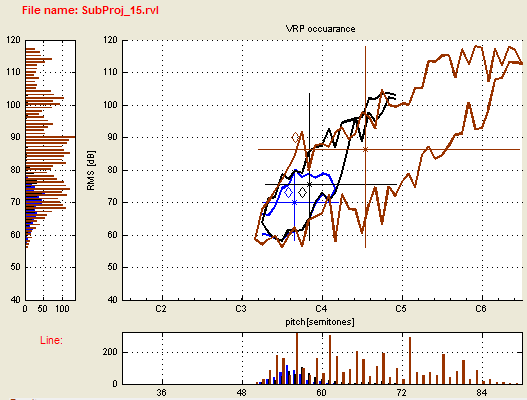
\includegraphics[width=0.8\textwidth, height=8cm]{img/autoreferat-vrp.png}
%    \caption{Voice Range Profile shows maximum and minimum intensity levels (y-axis) across the vocal range (x-axis) of normal speech (area surrounded by blue line) and singing (area surrounded by brown line).
%    }
%    \label{fig:vrp}
%\end{figure}
%
%%Another method that is used to analyze vocal chords is laryngoscopy. The videostroboscopy and high speed video in laryngoscope methods produce videos showing real movement of vocal chords. The videokymography method, introduced by Švec et al., complements the videostroboscopy. It allows the visualizing and analyzes of the movement of vocal cords. These movements are recorded by a high speed camera and an new image constructed from selected line of recorded video, which can be shown on standard TV or monitor using low frequency \cite{Svec1996,Svec2007}. 
%
%%In the case of a recorded sound and further analysis, there is a question about how such a service can be integrated in a grid computing or cloud computing environment in order to provide access to a complex application for non-technical voice specialists. Additionally, analytical software was already developed and calibrated for selected types of microphones in the MS Windows platform by Frič et al. \cite{Fric2007,Fric2012}. Therefore, I proposed and implemented a method that provides remote access to the analytical software. Section \ref{sec:methodsvoice} describes how the analytical software was customized with a remote desktop protocol (RDP)\nomenclature{RDP}{Remote Desktop Protocol}. Results are described in section \ref{sec:resultsvoice}. A similar approach can be used for processing  video recordings from a laryngoscope, however, the practical limits are discussed in section \ref{sec:conclusion}. 
%
%%\subsection{Methods for Remote Analysis of the Human Voice}
%\label{sec:methodsvoice}
%Terminal access to some remote computational capabilities, e.g., remote command-line or remote execution, is another integration strategy that is used for some remote infrastructures. Secure Shell (SSH) is used to establish a secure channel via an unsecured network (e.g., the Internet) from an SSH client to a SSH server. This is a basic method that is used to access a grid computing infrastructure. 
%Remote Desktop Protocol (RDP)\nomenclature{RDP}{Remote Desktop Protocol} is a proprietary protocol that is used for desktop sharing. It was primarily developed in a Microsoft Windows platform, however, today, clients and servers exist for several other platforms. Next to remote command-line, remote execution allows the accessing of remote graphical desktop environments. 

%
%%The computation of frequencies and amplitude from the recorded samples utilizes the effective Fast Fourier Transformation, which has time complexity $O(n\log(n))$. The benefit of deploying such an application in distributed infrastructures is the immediate access to updated software. Additionally, a collection of anonymized records of voice samples and results are very useful for further research and education. The possible disadvantage is the need to access to Internet.
%
%%This type of application can be packaged as a virtual machine template and configured within different types of cloud infrastructures. Together with a script or web portal, the on-demand deployment can be automated. The client part (RDP client) needs to connect to the appropriate instance. The results of such a deployment are discussed in section~\ref{sec:resultsvoice}.
%
\section{Computational physiology}
\label{sec:models}
A mathematical formalization of the fundamental knowledge and relation among a biological system – a mathematical model - is used as a base abstraction in order to utilize the current discoveries of the genomics and proteomics. It is also used to formalize the knowledge and construct a "Physiome Model". By  definition, a model is the simplification of a complex reality. Constructing the models and integrating them into a complex entity, which can be used for further purposes, is schematically illustrated in Figure \ref{fig:modeling}. 

\begin{figure}[ht]
    \centering
    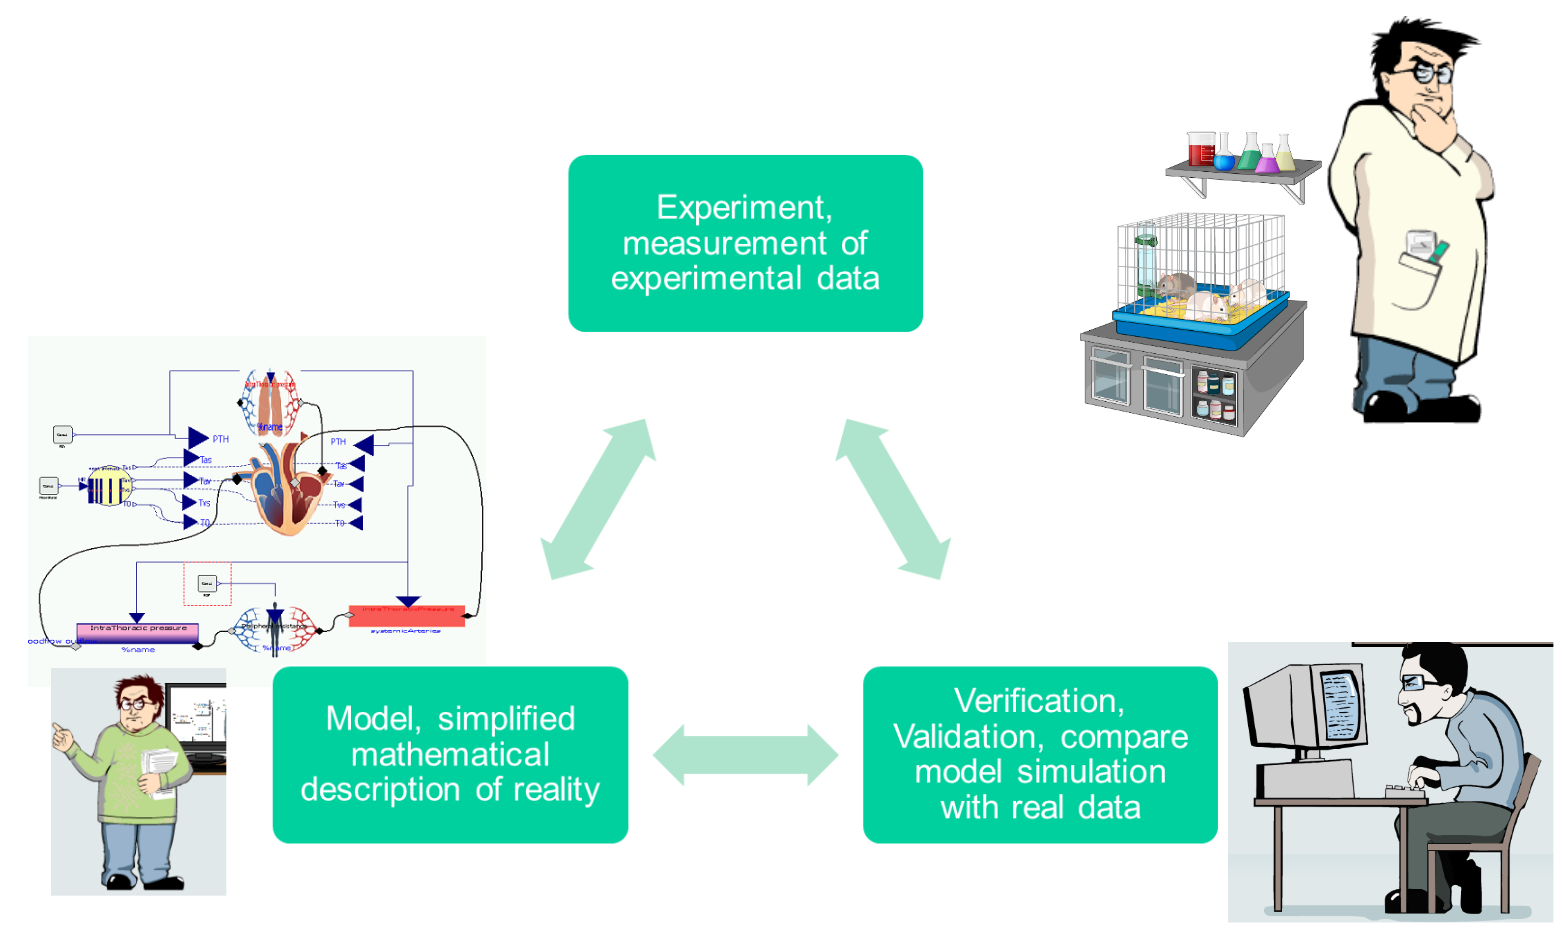
\includegraphics[width=1\textwidth]{../chapter3/modeling.png}
    \caption{Schematic illustration of the scientific process. The experiments produce data that are interpreted and a hypothesis is formalized as a model. Validation compares the model simulation with the experiment, if the model satisfies the criteria -- if it is in agreement with real experiments -- then the validated model can be used for other purposes. 
    }
    \label{fig:modeling}
\end{figure}

There are used several technologies in order to implement a formalized model of physiology. Within the work of this thesis a Modelica language was choosen, because it was identified as robust to maintain most complex models of human physiology in understandable way \cite{Kofranek2011hummod}. Additionally, a library Physiolibrary developed by Matejak et al. (21.) %\cite{Matejak2014} 
was enhanced and used especially within the hydraulic domain components as listed in Table \ref{table:physiolibrary}. 

\begin{table}[!ht]
\small
\centering
\begin{tabular}{m{1.0cm} m{10.2cm}}
%\begin{tabular}{m{1.2cm} m{13.5cm}}
\hline
Icon & Description \\
\hline
%\begin{tabular}{m{1.5cm} m{12.7cm}}

\includegraphics[scale=0.8]{HydraulicPorts.png} & Acausal hydraulic connectors -- the MODELICA tool generates "Kirchhoff law" analogy for all non-flow variables $p_1 .. p_n$ (pressure) and "flow" variable $q1..q_n$ (flowrate):\\
 & $ \label{eq:con1} p_1 = p_2 =... = p_n$ \\
 & $ \label{eq:con2} \sum_{i=1}^{n} q_i = 0$  \\
\hline
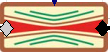
\includegraphics[scale=0.4]{resistance.png} & Hydraulic Resistor--characterized by $G$--conductance parameter (reciprocal value of resistance $G = 1/R$) and defined by relation among quantities from both hydraulic connectors, $q$--flowrate and $(p_{out} - p_{in})$ --pressure gradient:\\ 
 & $ \label{eq:resistor} q = G *(p_{out} - p_{in}) $ \\ \hline

\includegraphics[scale=0.4]{elasticity.png} & Elastic compartment--characterized by parameters: $C$--compliance (reciprocal value of elastance $C=1/E$), $V_0$--unstressed volume, $p_0$--external pressure. The relation among $p$--pressure, $V$--volume and $q$--flowrate are:\\ 
& $ \label{eq:compliance}p-p_0 = \left\{   
  \begin{array}{l l} 0 & \quad \text{if } V \text{\textless} V_0 \\ 
    \frac{V-V_0}{C} & \quad \text{otherwise}
  \end{array} \right.$ \\
 & $ \label{eq:flowrate}\frac{{\rm d}V}{{\rm d}t} =  q$ \\ 
 \hline
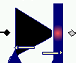
\includegraphics[scale=0.5]{valve.png} & Valve is characterized by $g_on$ -- inflow, $g_off$ -- backflow conductance and $P_{knee}$ forward threshold pressure. The relation for $dp$ pressure gradient and $q$ flowrate between the two connectors are:\\
 & $dp = \left\{ \begin{array}{lr} pass/g_{on} +P_{knee} & \text{for } pass >0 \\
   pass + P_{knee} & \text{otherwise} \end{array} \right. $ \\
% & $dp = \left\{ \begin{array}{1 1} pass/g_{on} +P_{knee} & \text{for } pass >0 \\
%   pass + P_{knee} & \text{otherwise} \end{array} \right. $ \\
 & $q = \left\{ \begin{array}{lr} pass + P_{knee} & \text{for } pass > 0 \\
     pass \times g_{off} +P_{knee} \times g_{off} & \text{otherwise } \end{array} \right. $ \\  
\hline
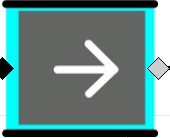
\includegraphics[scale=0.2]{inertia.png} & Inertia element is characterized by the $I$--intertance parameter and the relationship between pressure and solution flow of the two connectors:\\
 & $ q_{out}=-q_{in} $ \\
 & $ \frac{{\rm d}q_{in}}{{\rm d}t} = \frac{p_{in}-p_{out}}{I} $ \\
\hline
 \end{tabular}
 \caption{Icon and description of hydraulic components of Physiolibrary (21.). These are used, e.g., in order to model cardiovascular system.}
 \label{table:physiolibrary}
\end{table}

Once the model is formalized and constructed, a further problem is to estimate the model parameters so that the model reproduces a real world system. Without any further knowledge about the model, the problem of parameter estimation (or system identification) was shown to belong to the \emph{NP-complete} problems \cite{Hofmann2005}, which implies that the best known exact algorithm solving this problem has exponential time complexity. The heuristic methods (evolution strategies), randomization methods (Monte-Carlo method) and others are commonly used in order to find at least some parameter estimation in a reasonable time. Therefore, in further  work of this thesis an evolution strategy, genetic algorithm, was choosen as most robust for common models and system was proposed and implemented, which integrates this algorithm implemented in MATLAB environment and model simulation implemented in Modelica language.

The specific model of a studied system that is implemented in Modelica can be simulated in some Modelica tool. Or can be exported into a standard Functional Mockup Unit (FMU)\nomenclature{FMU}{Functional Mockup Unit}. Functional Mockup Interface (FMI)\nomenclature{FMI}{Functional Mockup Interface} defines FMU as a standardized XML\nomenclature{XML}{Extensible Markup Language} metadata description, packaged together with a binary library .DLL (or .SO), following a standardized API, published by Blochwitz et al. \cite{Blochwitza}\footnote{\url{https://www.fmi-standard.org/} accessed February 2015}. This API can be used to get/set values of model variables and to simulate the model.


%
%%The measurements are carried out in laboratories or in hospitals. Lumped parameter models are usually represented as ordinary differential equations and differential algebraic equations. They characterize the reality as a topology of discrete elements. The imaging methods for processing and analysis (section \ref{sec:imaging}) are used to construct 3D models from segmentation and generate mesh representations that are connected to physical principles. 


%
%%The application of mathematical modeling techniques towards biomedical research is sometimes called systems biology. This approach combines the reductionism and integration, as denoted by Kohl et al.\cite{Kohl2010}. Application towards clinical practice includes the quantification of the diagnostic index or treatment strategy. It is a goal to develop tools, database models and methods of several Physiome projects, e.g., VPH-Physiome project presented by Hunter et al.\cite{Hunter2009}.
%
%One of the earliest complex and integrative modeling efforts was a model of circulation and its regulation, which was published by Guyton et al. in 1972 \cite{Guyton1972}. It continues as a "Human Model" or "HumMod" via derivative and technological upgrades, as introduced by Hester et al. \cite{Hester2011systems,hester2011}, with a focus on integration efforts. A different approach of modeling the human physiology is to construct a database of smaller models, which focus on some particular physiological phenomenon. For example, the NSR Physiome project introduces a  JSIM\footnote{JSIM: \url{http://www.physiome.org/jsim/} accessed January 2015} Java-based simulation system in order to support modeling in  physiology. A repository of several hundred models was published using this system \cite{Butterworth2014}. A similar effort is made by the IUPS Physiome project and repositories of the models are  based on XML standard languages CellML and FieldML \cite{Hunter2004,Yu2011}. The Systems Biology Markup Language (SBML) is used for modeling a biological system at the level of biochemical reaction and regulatory network. Another database collects several hundreds of curated and non-curated models \cite{Hucka2004,LeNovere2006}. These in-house domain-specific language and tools (although standardized by several organizations) like JSIM, CellML and FieldML, SBML or HumMod, have reached their capabilities for representing complex models. Only the HumMod achieved the integrative approach, building a complex integrative model of human physiology using a lumped parameter approach. However, as the HumMod modeling technology is maintained by a small team of experts, it is not used in broader physiology community. Other authors use commercial or industry standard tools for mathematical modeling and computing. For example, Kofranek et al. described Guyton's 1972 model in MATLAB\textsuperscript{\textregistered} Simulink \cite{Kofranek2010} and the derivative HumMod in acausal object-oriented Modelica language \cite{Kofranek2011hummod,kofranek2013hummod}.
%
%

%
%
%\subsection{Modeling Methodology}
%\label{sec:methodsmodels}
%
%
%%The methodology of formalizing mathematical models is influenced by the abilities of underlying modeling language that is used. 
%%JSIM, CellML, SBML or HumMod are domain specific languages and the tools that are primarily developed within physiological or systems biological communities. 
%%Other authors use commercial or industry standard tools for mathematical modeling and computing. For example, Kofranek et al. described Guyton's 1972 model in MATLAB\textsuperscript{\textregistered} Simulink \cite{Kofranek2010} and the derivative HumMod in acausal object-oriented Modelica language \cite{Kofranek2011hummod,kofranek2013hummod}. Fernandez et al. described models of cardiovascular pulsatile system using MATLAB Simscape  \cite{FernandezDeCanete2013} and recently, in Modelica  \cite{FernandezdeCanete2014}.
%
%The Modelica language is an object-oriented, equation-based and acausal modeling language standardized and maintaned by the Modelica association\footnote{\url{http://www.modelica.org} accessed February 2015}.
%
%%finished writing of autoreferat 7th April.
%Therefore, I contributed to the modeling methodology beneficial for complex models, which key features are the acausal modeling technique and object orientation. This keeps the complex model structure decomposed into understandable and maintainable parts and allows the complexity of models like HumMod to be covered. 
%
%The paper \cite{Kulhanek2014Modeling} \emph{Modeling of Short-term Mechanism of Arterial Pressure in the Cardiovascular System: Object-oriented and Acausal Approach} in Appendix~\ref{app:modeling} published disputation about causal and acausal approach in using Modelica for modeling pulsatile cardiovascular system (CVS)\nomenclature{CVS}{Cardiovascular System} and possible enhancement for more complex models. 
%
%The paper \cite{Kulhanek2014mefanet} \emph{Simple Models of the Cardiovascular System for Educational and Research Purposes} in Appendix~\ref{app:simplemodelsd}, published detailed methodology of modeling lumped parameter pulsatile CVS in Modelica. 
%
%A common guide to the Modelica language and its capabilities can be found an the published works of Fritzson \cite{fritzson2002} and in the on-line works of Tiller \cite{Tiller2014}.
%
%
%\subsection{Identification of physiological systems}
%\label{sec:estimation}
%


% This procedure is sometimes called system identification and the objective of the parameter estimation is usually to minimize the following function (to find the least amount of differences between the predicted and measured values):
%\begin{equation} \label{eq:parameter} 
%f( \vec{p} ) = \sum_{i=1}^{n} ( M(t_{i},\vec{p} ) - d(t_{i}) )^2 \to min  
%\end{equation} 
%where $\vec{p}$ is the vector of values of parameters, $M(t_{i},\vec{p})$ is model simulated at time $t_{i} $ with the given parameter values $\vec{p}$ and $d(t_{i})$ is the measured experimental value at time $t_{i}$. 



%global optimization methods must be used in general, and ,
%, e.g. based on brute-force search -- trying all possible values of the parameters and simulate the model with them, finding the minimum of the objective function (\ref{eq:parameter}).
%Further reading about parameter estimation and system identification can be found in published works edited by Eykhoff \cite{Eykhoff1981}, or in the published works of Khoo \cite[p.~159]{khoo2000}.
%


%Evolution strategies have been identified as robust, having the potential to utilize parallel computing methods \cite{Moles2003}.
%
%Parameter estimation and further analysis methods are part of specialized mathematical software. For example, Pruet et al. used Metropolis algorithm to produce a distribution of parameters in order to calibrate a model of the human cardiovascular physiology. This was further tested against the predictive ability of circulatory failure and statistical methods were used with the software Wolfram \textit{Mathematica} \cite{Pruett2013}. The iterative improvement method in the MATLAB Simulink\textregistered ~was used by Takahashi et al. in their estimation of two parameters of a simple cardiovascular model \cite{Takahashi2013}. Furthermore, Abbas et al compared several methods in their estimation of multiple parameters of a cardiovascular system in MATLAB Simulink\textregistered \cite{Abbass2012}.
%
%Maffioletti et al. published a GC3Pie framework, which utilized evolutionary algorithms. They introduced workflow to identify parameters of models for economical predictions, using grid computing infrastructure \cite{maffioletti2012computational}. Humphrey et al. calibrated hydrology models, utilizing a commercial Windows Azure cloud computing infrastructure and achieved significant speedup \cite{Humphrey2012}.
%
%\subsection{Methods for Parameter Estimation}
%\label{sec:methodsestimation}
%
%\begin{figure}[htb]
%    \centering
%    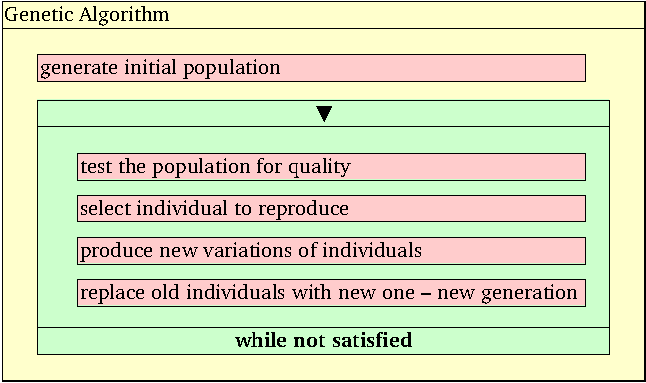
\includegraphics[page=1]{chapter3/GA-kopenogram-crop.pdf}    
%%    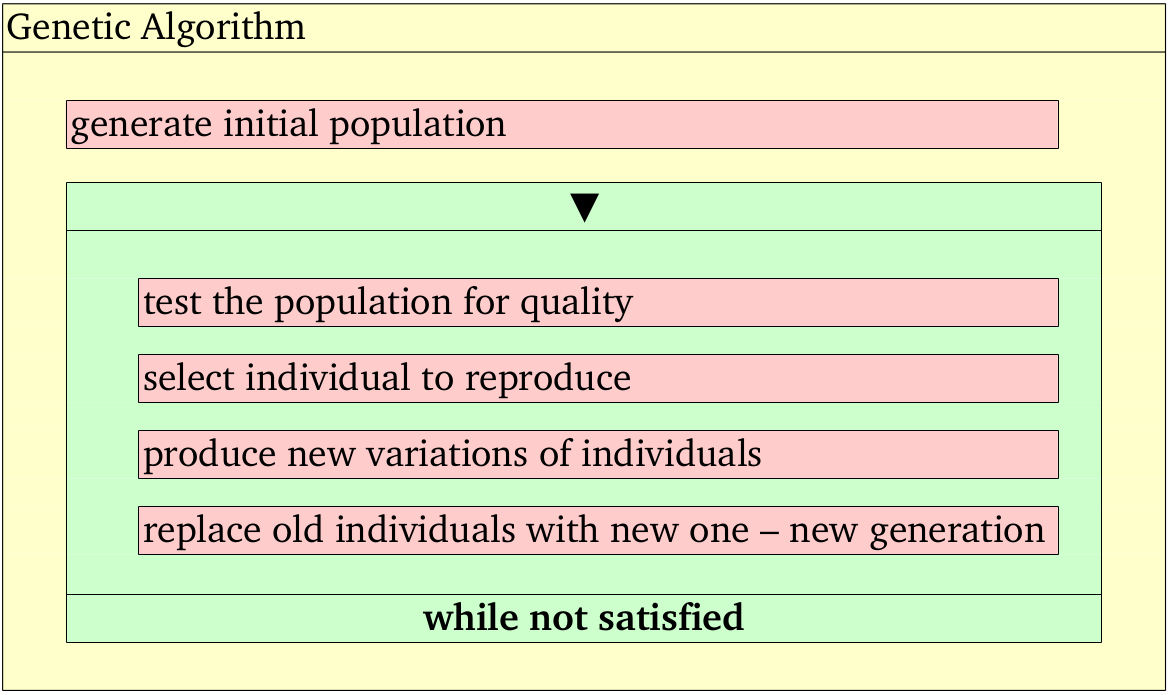
\includegraphics[width=0.5\textwidth]{chapter6/GA-kopenogram.png}
%    \caption{Kopenogram of a genetic algorithm. 
%    }
%    \label{fig:GA-kopenogram}
%\end{figure}
%
%An evolutionary algorithm can be used as a heuristic strategy for finding global minimum or maximum. It can also be used to estimate the parameters of a model. A genetic algorithm is a type of evolutionary algorithm, which encodes individuals as binary string. It was introduced by the likes of Holland\cite{Holland1975}. These algorithm steps are schematically presented in Figure \ref{fig:GA-kopenogram}.
%
%\begin{figure}[htb]
%    \centering
%    \includegraphics[page=2]{chapter3/GA-kopenogram-crop.pdf}    
%%    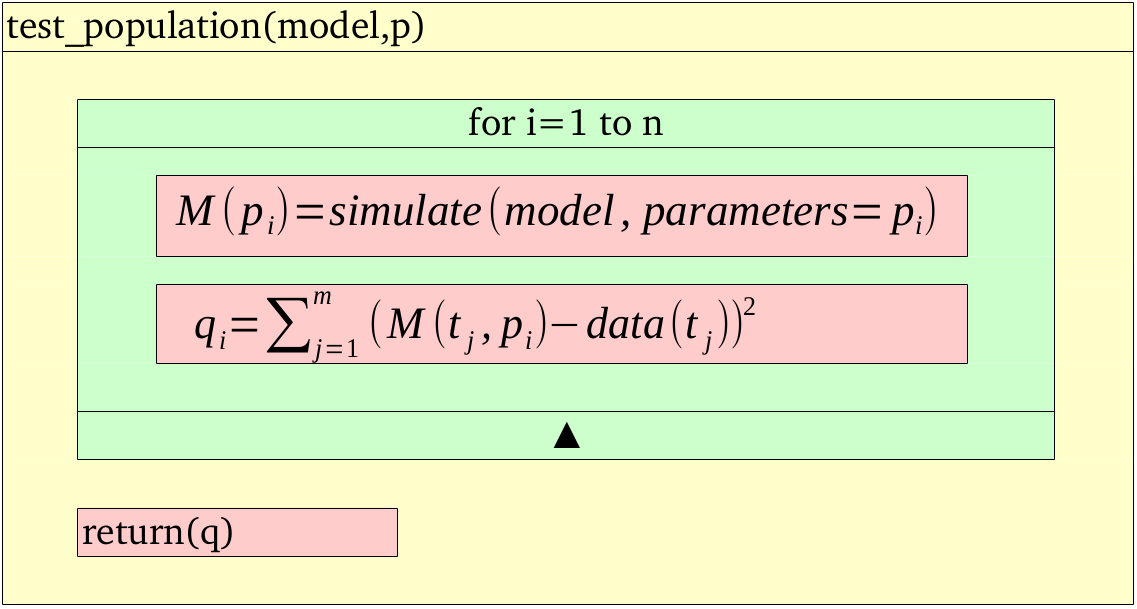
\includegraphics[width=0.5\textwidth]{chapter6/GA-kopenogram2.png}
%    \caption{Kopenogram of the specific test of a population for quality, in the case of parameter estimation used by a genetic algorithm. The model is simulated according to individual $i$ with parameters $p_i$ and the quality $q_i$ is counted per the objective function \ref{eq:parameter}.
%    }
%    \label{fig:GA-kopenogram2}
%\end{figure}
%
%The iteration within the loop "$\blacktriangledown \ldots$ \emph{while not satisfied}" depends on the previous iteration and, thus, it cannot be parallelized. However the \emph{test the population for quality} has an algorithmical structure in Figure \ref{fig:GA-kopenogram2} for the parameter estimation. Each iteration in the loop "\emph{for i=1 to n}" is independent and, therefore, loop parallelism (section \ref{sec:parallelprogramming}) can be utilized and implemented here.
%
%\subsubsection{Architecture of System for Parameter Estimation}

%
%The parallelization is implemented using threads. For this, in \emph{test\_population} method is used, which, within a loop, follows a fork/join pattern -- the created threads simultaneously ask for simulation results with a parameter set and the main process waits until all of the results are returned before computing the full vector of quality evaluation $q$.
%
%Model specific FMU is packaged with a .NET ServiceStack framework\footnote{\url{https://servicestack.net/} accessed February 2015} and it exposes a simulation functionality as a RESTful web service, which can be accessed and orchestrated by the \emph{test\_population} algorithm. The implementation of genetic algorithm is reused from MATLAB \texttrademark Global Optimization Toolbox\footnote{\url{http://www.mathworks.com/products/global-optimization/} Matlab Global Optimization Toolbox, accessed March 2015} and, with a database of results in a SQL database, is integrated with an ASP.NET web application. This presents a web user interface and functionality to a user. Section \ref{sec:resultsestimation} describes the results of applying the methods and deploying the designed system in a local cluster and cloud computing infrastructure.
%
%\subsection{Parameter Sweep}
%\label{sec:sensitivity}
%After the parameter estimation, further problem arise regarding the structural identifiability and analysis of sensitivity to the estimated parameter values\cite[p.~176]{khoo2000}. 
%
%\begin{figure}[hbt]
%    \centering
%     \includegraphics[page=4]{chapter3/GA-kopenogram-crop.pdf}    
%%    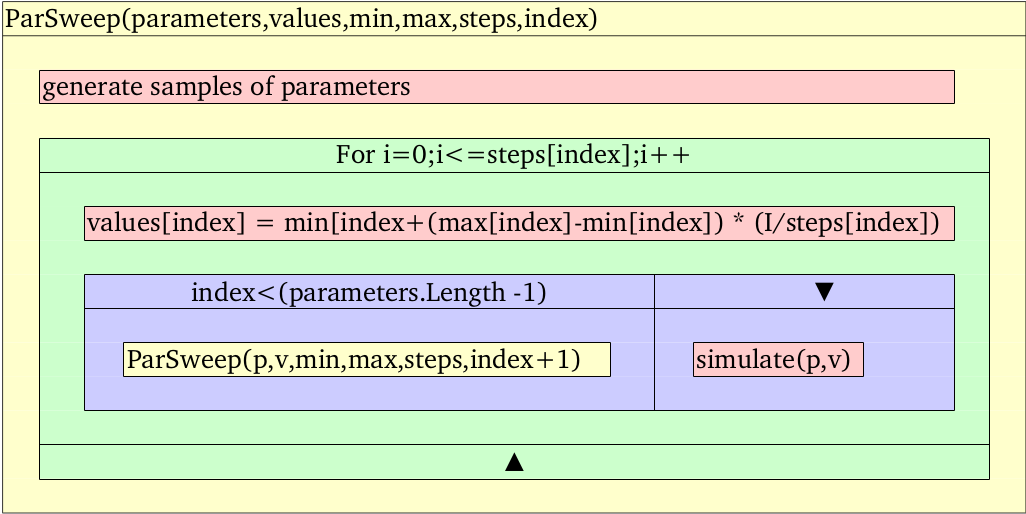
\includegraphics[width=1\textwidth]{chapter3/paramsweepkop.png}
%    \caption{Kopenogram of a recursive parameter sweep algorithm. $p$,$v$,$min$,$max$ and $steps$ are arrays with the same dimension that hold the parameter name, value, starting and stopping value and number of steps that have to be performed between the starting and stopping value per each $index$.    
%    }
%    \label{fig:paramsweep}
%\end{figure}
%
%Parameter sweep (PS) is one of the techniques that is used for a sensitivity and uncertainty analysis, which is based on the changing selected parameters, simulating whole model and quantifying the change on model behavior with different parameters. An uncertainty and sensitivity analysis tries to determine how a change in the value of a parameter  contributes to the model output and how the estimation of parameter values is robust against errors of real data measurement. The various methods for carying out an uncertainty and sensitivity analysis have been published, e.g., in reviews by Helton et al. \cite{Helton2006} or in publications by Saltelli et al.\cite{Saltelli2004,Saltelli2008}. 
%
%The recursive algorithm of a parameter sweep for exploring parameter space (in Figure \ref{fig:paramsweep}) generates a tremendous number of simulations. Presuming that \emph{simulate} operation takes a constant time for any parameters (which, in general, is not true), the time complexity of PS is exponential $O(\prod_{i=1}^{n}) \text{steps}_i) \approx  O(k^n)$ where $k=\max_{i=1}^n(\text{steps}_i)$ and $n$ is number of parameters to be swept. For example, for 1~000 values for each parameter: $O(1000^n)$. The large number of distinct simulation can take a tremendous ammount of time on a single computer. However, in contrast to parameter estimation, each simulation is independent and a PS algorithm is determined as embarrassingly parallel. It is implemented in many grid computing projects and workflows, e.g., P-Grade portal, as published by Kacsuk et al.\cite{Kacsuk2011}.
%
%A system was proposed with customized BOINC platform\cite{Anderson2004}\footnote{\url{http://boinc.berkeley.edu/} accessed February 2015}. The task parallelism and master/worker programming model (mentioned in section \ref{sec:parallelprogramming}) is utilized. The Modelica model exported as FMU for Windows platform is integrated with BOINC wrapper. As a whole, it is integrated into BOINC platform, which is deployed on a server, as seen in Figure \ref{fig:paramsweeparch}. 
%
%\begin{figure}[htb]
%    \centering
%     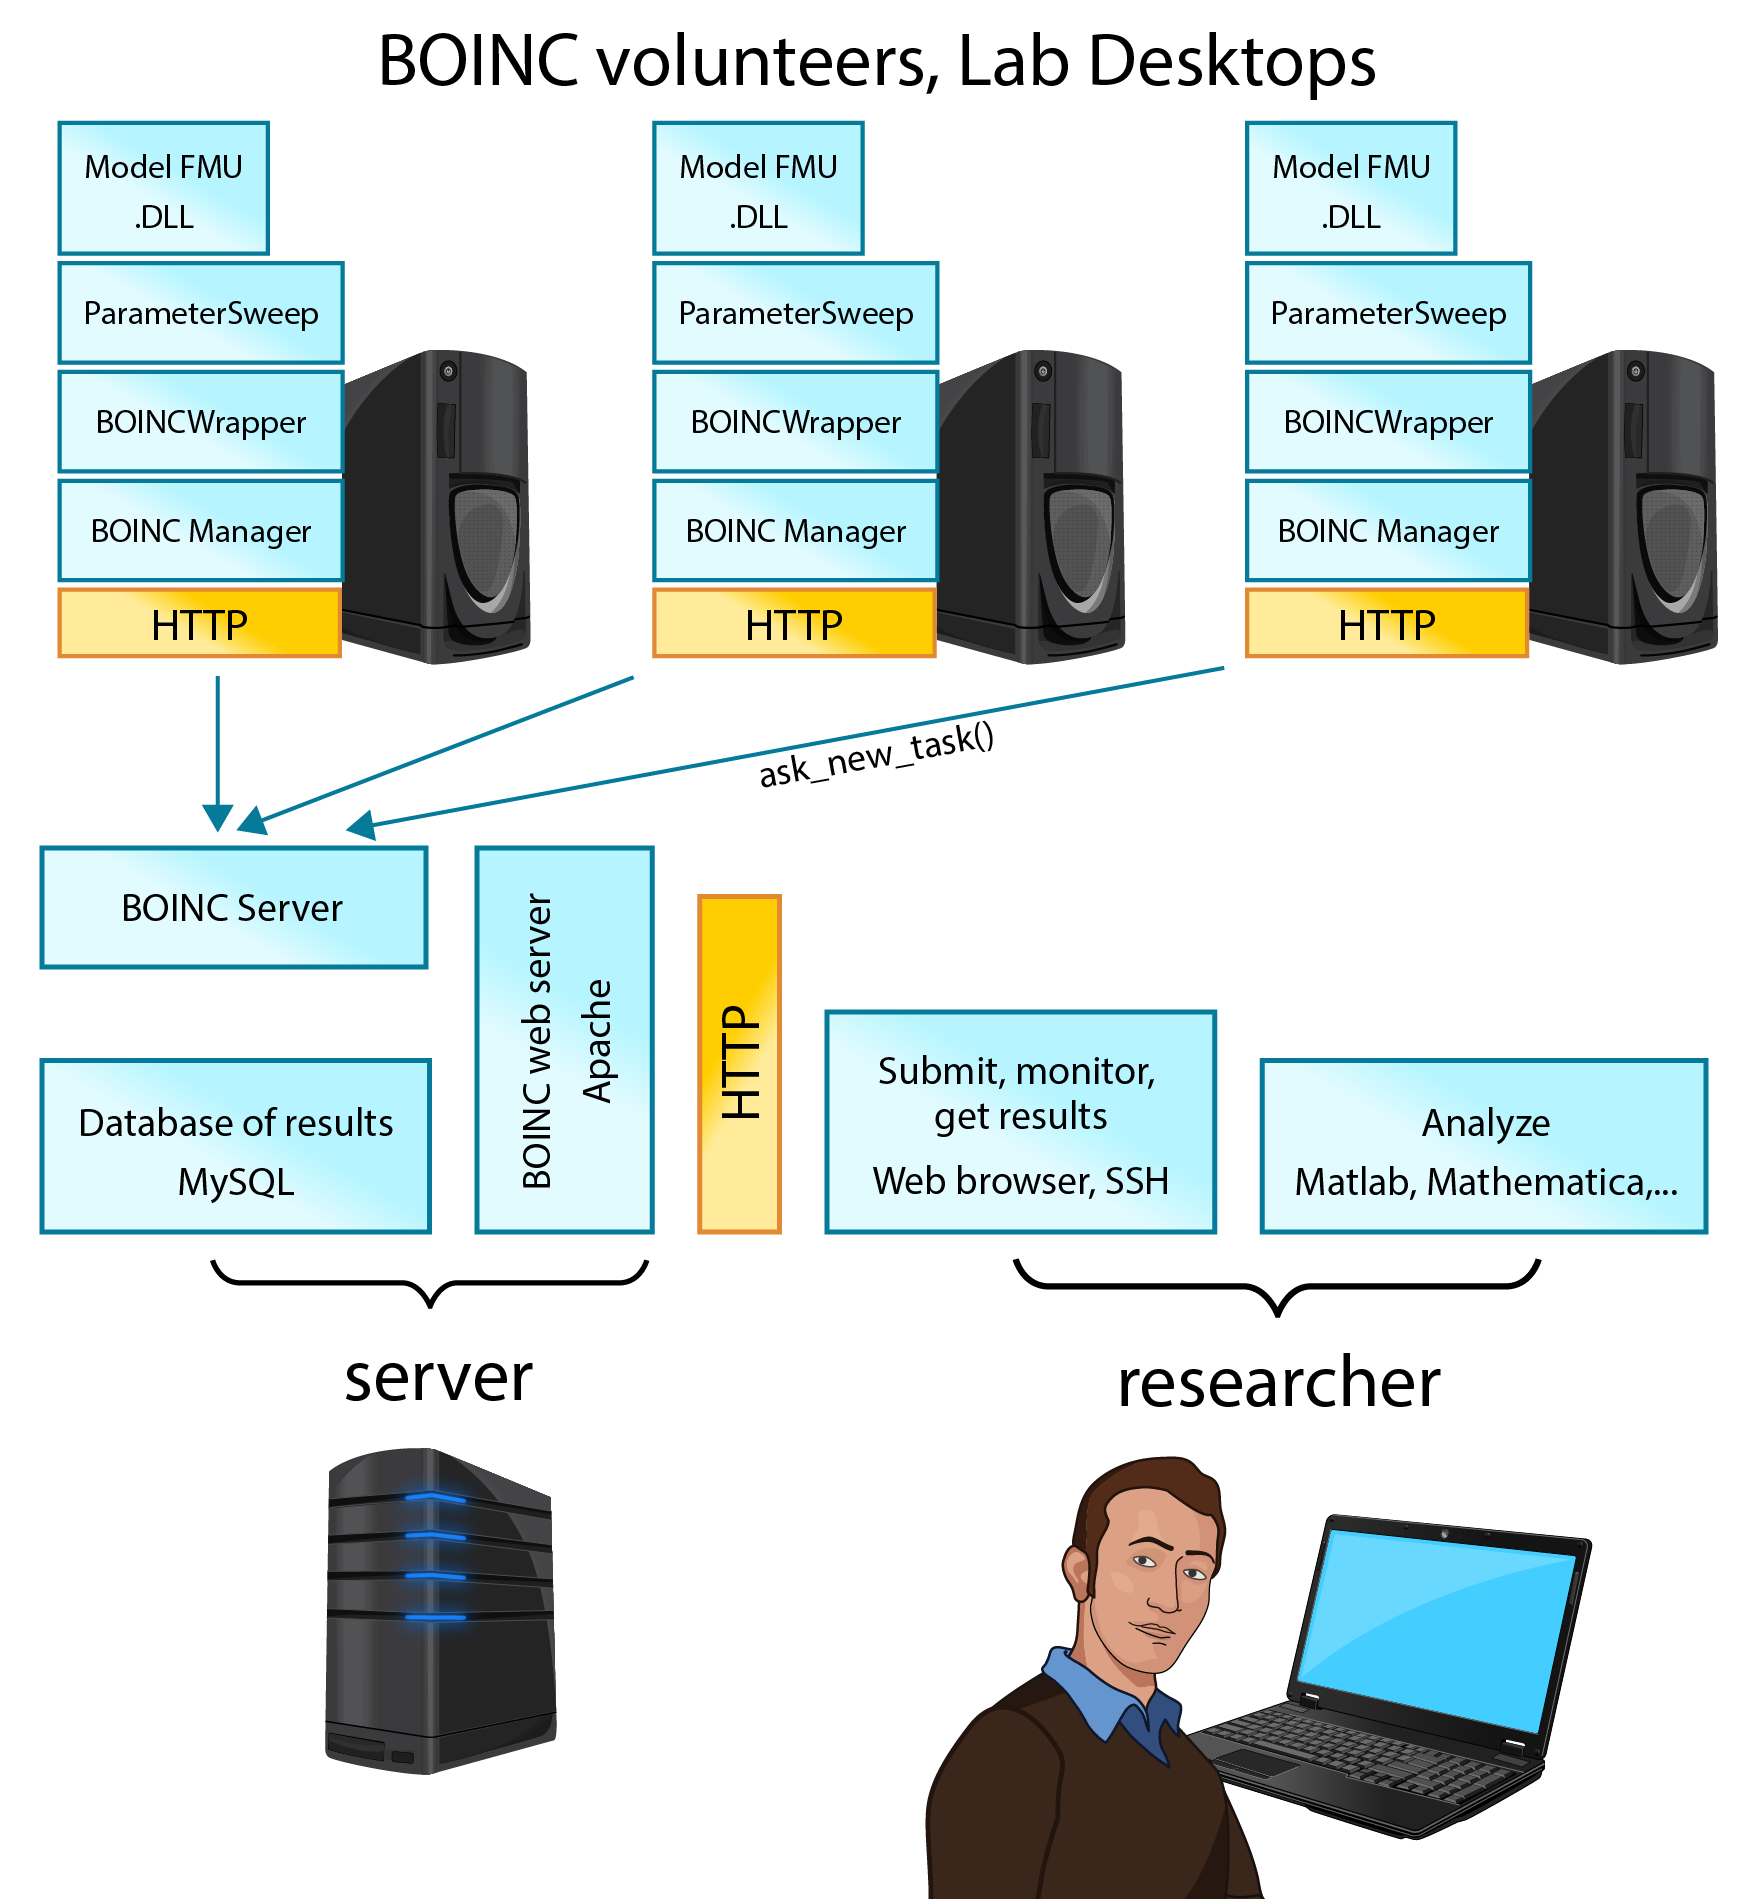
\includegraphics[width=0.75\textwidth]{img/chapter3-architekturaparamsweep-01.png}    
%%    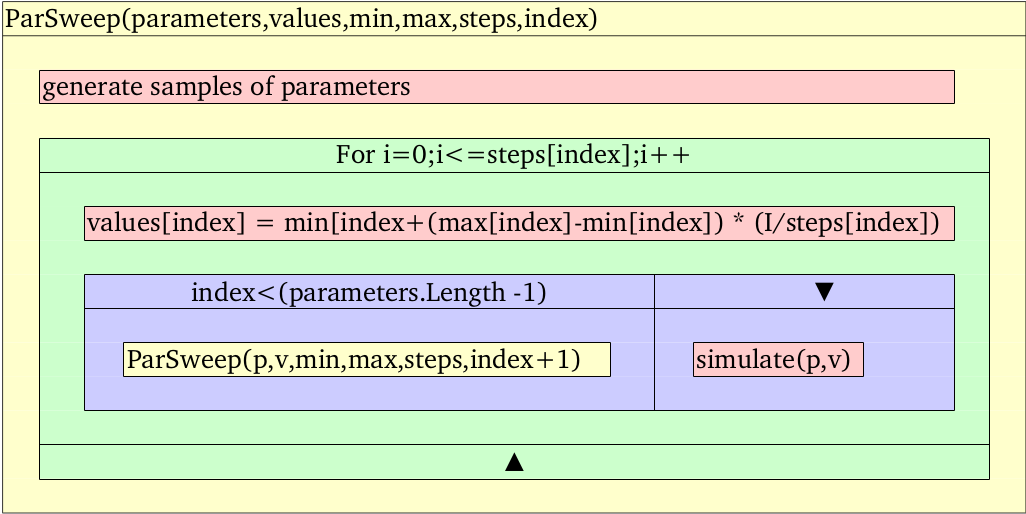
\includegraphics[width=1\textwidth]{chapter3/paramsweepkop.png}
%    \caption{Architecture of a parameter sweep integrated into BOINC framework. The whole parameter space is divided into smaller spaces which are resolved by the BOINC workers}
%    \label{fig:paramsweeparch}
%\end{figure}
%
%The results are described in section \ref{sec:resultsestimation}.
